\documentclass[spanish, fleqn]{article}
\usepackage[english]{babel}
\usepackage[utf8]{inputenc}
\usepackage{amsmath}
\usepackage{amsfonts}
%\usepackage{wasysym}
%\usepackage{mathrsfs}
\usepackage[colorlinks, urlcolor=blue]{hyperref}
\usepackage[top = 2.5cm, bottom = 2cm, left = 2.5cm, right = 2.5cm]{geometry}
\usepackage{fancyhdr, graphicx}
\usepackage{caption}

\renewcommand{\headrulewidth}{0pt}
\fancyhead[L]{
\includegraphics[width=3cm]{Logo_INFO.png}}
\fancyhead[R]{
\includegraphics[width=3.2cm]{Logo_UTFSM.png}}

\begin{document}
	\thispagestyle{empty}
	\newpage
	\null
	\vskip 4em
	\begin{center}
		\textsc{\Large Universidad Técnica Federico Santa María.}\\[0.4cm]
		\textsc{\Large Sistemas y Organizaciones.}\\[0.2cm]
		\textsc{\LARGE Análisis de la Estructura Organizacional.}\\[1.2cm]
	\end{center}

	\thispagestyle{fancy}

	El artículo leído, ``La estructura organizacional no es fija'' del Mercurio
	21 de Julio del 2014, nos habla de cómo las organizaciones varían debido a
	los cambios del ambiente, por ellos se puede hacer necesario la modificación
	de la misión de la misma y así también cambia su estrategia.\\
	En este informe se analizarán los diversos factores, descritos por el articulo,
	a tener en cuenta para analizar la estructura de una de las organizaciones
	de mayor influencia en mi vida y la de muchos amigos, la Universidad
	Técnica Federico Santa María.
	\begin{figure}[h!]
		\centering{ 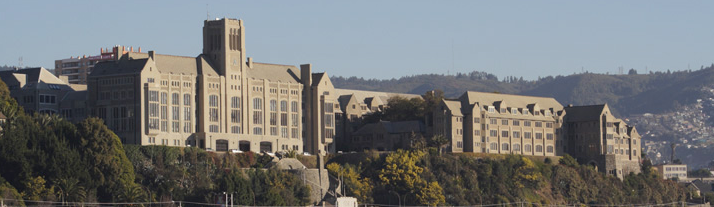
\includegraphics[width=15cm]{uni.png} }
		\caption*{Universidad Técnica Federico Santa María, Casa Central.
				 Fotografía propiedad de UTFSM.}
	\end{figure} \\
	\textbf{Analisis del Entorno:} El artículo plantea que analizar el entorno y
	reaccionar ente ello es uno de los factores más importantes a la hora de decidir
	si debemos cambiar la misión y estrategia de una organización. La universidad
	debe estar bien informada sobre la problemática estudiantil que golpea
	fuertemente a nuestro país. Creo que en éste aspecto no existen mayores
	problemas, quizás sea por la contingencia de las medidas tomadas por parte
	del estado, pero he notado que la situación es comúnmente hablada y analizada
	al menos por los estudiantes y algunos profesores, aún así nos falta saber 
	que medidas se tomarán para enfrentar estos cambios y si se hace necesario
	un cambio en la misión y estrategia de la universidad.\\[0.1cm]
	\textbf{La organización del Siglo XXI:} Según el articulo las organizaciones
	actuales deben lidiar con algunos factores que han tenido un cambio notable
	en las ultimas décadas, entre ellos se destacan y analizan los siguientes:
	\begin{itemize}
		\item
			\textbf{Organización como Red:} Las organizaciones actuales deben
			buscar la especialización y olvidar la autosuficiencia. No es
			necesario que los servicios que no son del rubro de una organización
			sean manejados por ella. Actualmente existen diversas empresas que 
			se dedican exclusivamente a prestar servicios a otras organizaciones 
			y por ello generalmente son más competentes y eficaces. En el caso
			de la universidad, vemos como algunas partes de su funcionamiento 
			fueron delegadas a empresas especializadas, como ejemplo podemos 
			tomar el servicio de guardias o el casino. Aunque la organización
			pueda actuar como una red, también existen peligros a la hora de
			delegar demasiadas funciones, por ejemplo se puede perder la imagen
			de unidad dentro de la organización.
		\item
			\textbf{Fin de la estructura Piramidal:} Las estructuras jerárquicas
			de muchos niveles prácticamente ya no existen, en la actualidad se
			fomentan las jerarquías del tipo horizontal. En nuestra universidad,
			donde los alumnos podemos percibir mayormente este tipo de jerarquía,
			es en la división de departamentos. Creo que el funcionamiento interno
			de los departamentos es bastante bueno, pero, a la hora de relacionarse
			entre si existen muchos problemas. Para que un alumno de informática 
			haga un tramite de un ramo de matemáticas, por ejemplo, existen
			muchas trabas y burocracias. Cuando hay un problema con un ramo que 
			no es del departamento donde se estudia generalmente se necesitan
			autorizaciones de los departamentos afectados y por ultimo dirección
			de estudios, lo que demuestra una poca cohesión entre los departamentos.
		\item
			\textbf{Las nuevas generaciones:} Hoy en día se busca que las
			organizaciones no sean un limitante en la vida de los individuos que
			participan de ellas, las prioridades de las nuevas generaciones 
			sumadas a los factores anteriormente mencionados hacen que muchas
			veces los individuos no se sientan atados a la organización, no se
			conformen con lo que les ofrecen y varíen mucho a la hora de buscar
			especialización. Creo que esté factor es uno de los peores
			desarrollados por parte de la universidad, lamentablemente algunos
			departamentos siguen con la visión conservadora y se resisten al
			cambio a la hora de formar profesionales, no se interesan mucho en
			que es lo que busca cada alumno y simplemente siguen con lo que se
			hace desde hace mucho tiempo.
	\end{itemize}
	\thispagestyle{fancy}
	\textbf{Estrategia clara y conocida:} La difusión de la estrategia por parte
	de la organización es tan importante como la estrategia misma, todos los
	miembros deben estar enterados de los cambios para que así se trabaje en
	conjunto para lograrlos. En este sentido, en la universidad, los alumnos no
	tenemos mucho peso en la toma de decisiones por parte de los directivos por
	lo cual la información no llega directamente a nosotros y por ello no nos 
	sentimos importantes en este proceso. Actualmente existen diversas iniciativas
	por parte del alumnado para cambiar la situación, espero que de esta forma 
	tanto la toma de decisiones como el actuar acorde a ellas sea también nuestra
	responsabilidad.\\
	La universidad se encuentra en un periodo de cambio, tanto por el acontecer
	nacional como por los intentos de los alumnos en ser parte de algunas decisiones
	estratégicas que no solo afectan a la organización, sino que nos afectan a todos.
	\\[6cm]

	\vfil
	Hernán Vargas, 201073009-3 \hfill Tiempo SCT 03:35
\end{document}
